\setcounter{chapter}{-1}
\newcommand{\splunge}{\textcolor{red}{\bf SPLUNGE}}

\chapter{Getting started}
\label{cha:getting-started}

\minitoc

\section{Welcome}


Hello and welcome. In this first, introductory, lab we're going to
cover some of the basic things you'll need to know about the IT
infrastructure here in the School of Computer Science. Some of what we
tell you may well seem very obvious to you, and if that's the case
we'd ask you to be patient. Some other things might not be so obvious...

In this and every lab there will be academic staff and postgraduate students (demonstrators) around to help you. If you're stuck or find something that you really can't understand, then \emph{please ask for help.}; that's what the lab staff are here for, don't just sit there getting frustrated.

All the desktop PCs in the labs in the Kilburn building are
`dual-boot': they can be started up running either Linux or
Windows. This is for flexibility -- the labs for most course units  use
Linux, but some use Windows, and of course, outside the labs, you're free to use
whichever you prefer for any aspect of your studies. If you're not
familiar with Linux, don't worry. We'll be telling you a bit about it
in this lab, and you'll be looking at it in much more detail in subsequent labs.

\section{Using Windows}
\label{sec:using-windows}

We'll start with Windows, so the first thing we need to do is to make
sure your PC is running Windows. Have a look. If it is, 
and the screen looks like Figure~\ref{figure:welc-screen}, then you  you can move on to the end of this subsection and login.

If it isn't in Windows, you need to reboot the PC. To do
this, press \ttout{ctrl}, \ttout{alt} and \ttout{delete}.

This will probably cause strange messages to appear on the screen,
disappear, and be replaced by yet more strange messages. Be patient,
watch it all happen, and don't worry what it all means. After a while,
everything should settle down and the screen will look like
Figure~\ref{figure:welc-grub}.

\begin{figure}
\centerline{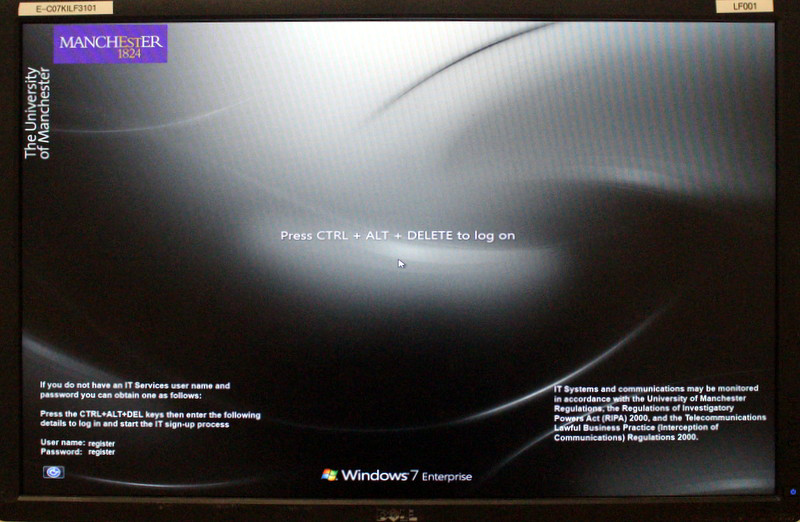
\includegraphics[width=15cm]{images/TH-win-welcome}}
\caption{The Windows7 Welcome screen.}
\label{figure:welc-screen}
\end{figure}

\begin{figure}
\centerline{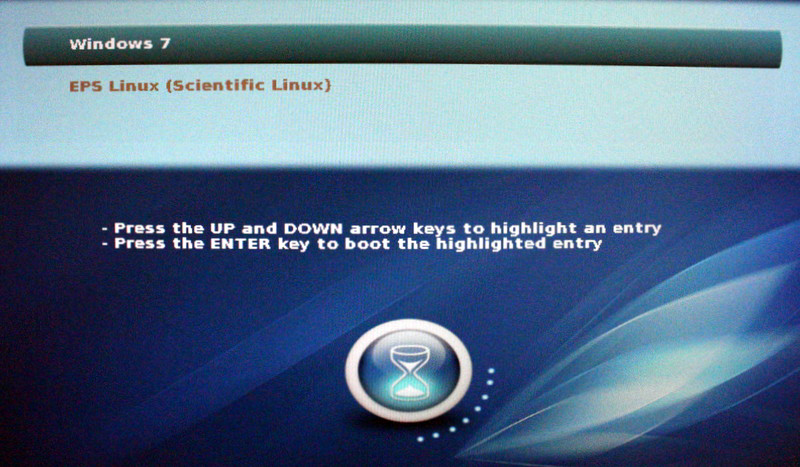
\includegraphics[width=15cm]{images/TH-grub-win}}
\caption{The boot selection menu screen.}
\label{figure:welc-grub}
\end{figure}

This is where you decide whether to start up Windows or Linux. If you do nothing, this will automatically boot into the default operating system after a fixed timeout period. In order to stop this timeout process, just press the space bar (or any other key). Now use the
up/down arrow keys on the keyboard to highlight the line
reading \ttout{Windows 7}, and press the enter key. After a short while, the Windows 7
welcome screen will appear, as shown in Figure~\ref{figure:welc-screen}. Now use the ctrl-alt-del chord again as instructed and you should see the Windows 7 login screen, as shown in Figure~\ref{figure:login-screen}.

\begin{figure}
\centerline{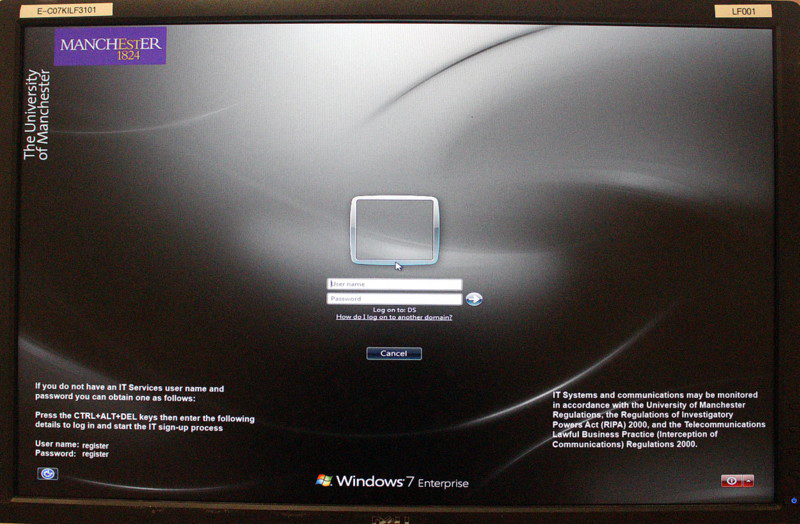
\includegraphics[width=15cm]{images/TH-win-login}}
\caption{The Windows 7 login screen.}
\label{figure:login-screen}
\end{figure}

To log in to your personal account, type in your username (this is an
8-character sequence starting with an `m'). Your password will
be the one  you set at registration. If your password doesn't work, or if you've forgotten it,
you need to fix this urgently. You can:

\begin{itemize}
  \item Find a machine running Windows and login with the username \ttout{register} and password \ttout{register}, then follow the instructions.
\item If you have access to a web browser, use the password recovery page at\\ \url{https://iam.manchester.ac.uk/recovery_login/overview}
%\item Visit the \verb|it.changes| Helpdesk in Kilburn Lower First area (Welcome Week, 09:00 -- 17:00)
\item Outside lab times, you can contact the University IT helpdesk (opening hours are Monday to Friday 9am to 5pm.) by phone on 0161 306 5544, or dial 65544 from a University internal phone; or you can visit the helpdesk in John Rylands Library (Building 55 on
the Campus Map), at the top of the escalator in the Blue 1 area.
\end{itemize}

Once you're logged in, go to your MyManchester page in a web browser, it's at

\url{https://my.manchester.ac.uk}

This page should look something like Figure~\ref{figure:welc-mymanchester}.

\subsection{Reading your email}

We use email extensively in the School, so it's vitally important that
you read your mail regularly -- at least once a day (and probably much
more often!). Follow the mail link (indicated by the green arrow in
Figure~\ref{figure:welc-mymanchester}) to access your email on the
University's Office365 system. This is a fully-featured system that
gives you 25GB of email storage space and an integrated calendar. You should
see a page looking something like Figure~\ref{figure:welc-mail365}.

Have a look around for a few minutes and check what mail you've
got. In particular, look for one with ``The Monday Mail'' in the
Subject line. This an important mail you'll receive every Monday
(hence the name) throughout your 3 or 4 years with us in the
School. The Monday Mail tells you what's going on each week in the
School. Take a moment to read it now. You can always read the Monday Mail, by the way, at the archive \urlnop{studentnet.cs.manchester.ac.uk/ugt/mondaymail/}

\begin{figure}
\centerline{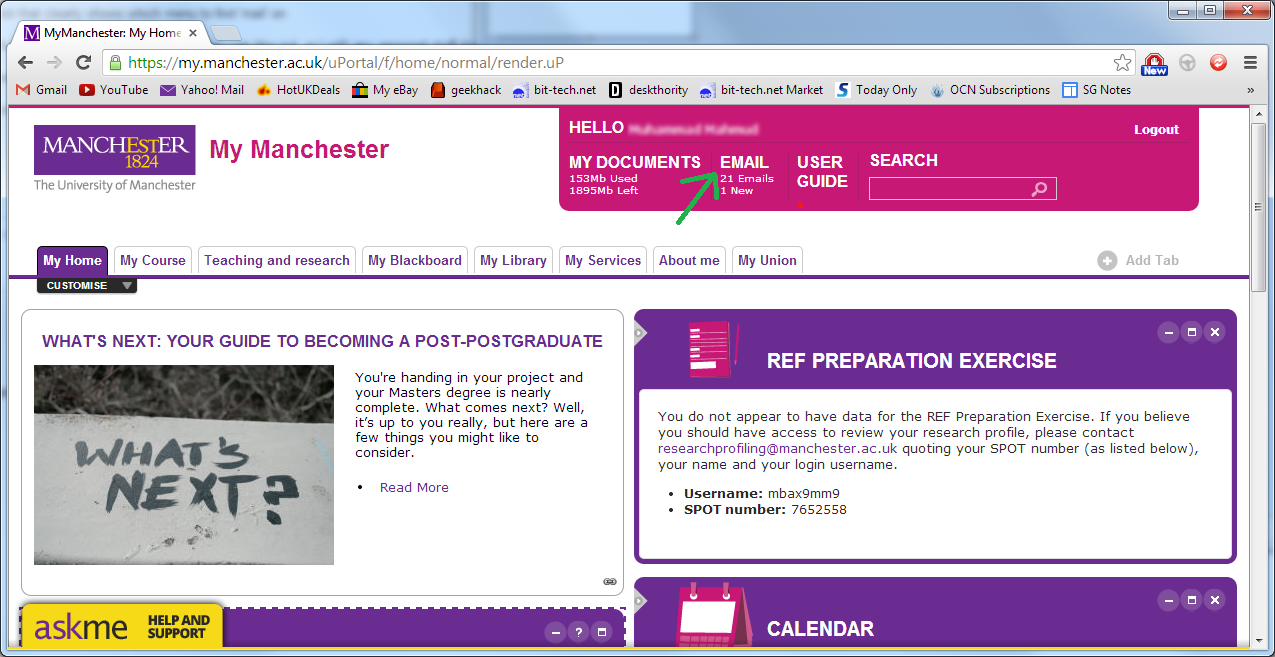
\includegraphics[width=15cm]{images/hamza-email-link.png}}
\caption{Your MyManchester page.}
\label{figure:welc-mymanchester}
\end{figure}

\begin{figure}
\centerline{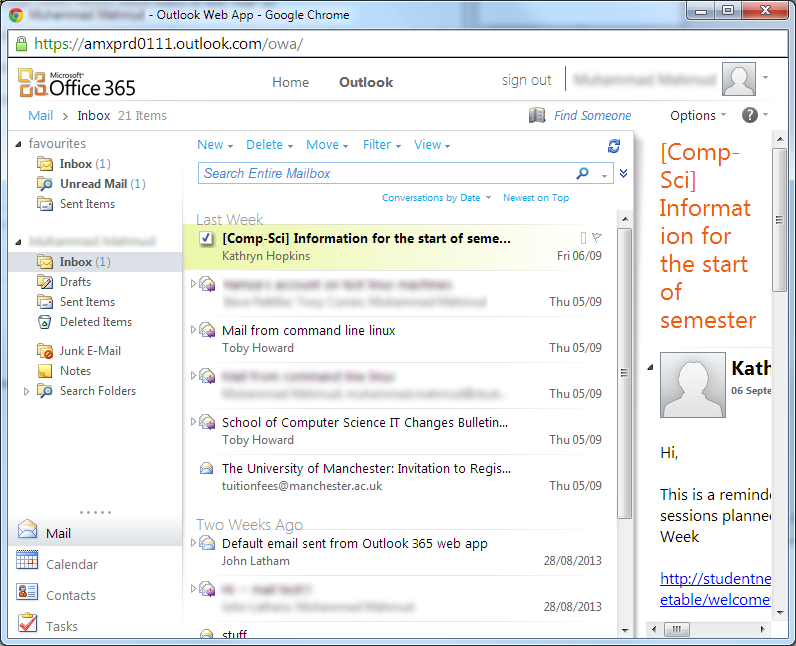
\includegraphics[width=15cm]{images/hamza-365-mail.png}}
\caption{Your Office365 email.}
\label{figure:welc-mail365}
\end{figure}

\label{sec:reading-your-mail}

Office365, like almost all modern email systems, supports the IMAP
protocol -- which means that you can access your mail from any device
that can run an IMAP mail client. Some examples of such clients are:
Mozilla Thunderbird, Mac Mail, Windows Live Mail and mail apps on mobile devices. No matter what
client you use, you need to tell it the appropriate settings. The mechanism for finding these setting can be found in our student wiki, which is located on the web at \urlnop{http://wiki.manchester.ac.uk/compsci/index.php/It.changes}. Look for the answer to question 'How do I configure my favourite IMAP mail client?'.

Once you've found the settings, use Office365 to email this information to yourself, to your
University account:

\url{firstname.lastname@student.manchester.ac.uk}

You'll need this information in a later lab so please don't delete this email after you've read it.

Finally, if you use an IMAP mail client on your phone or mobile
device, configure it to use the settings you've just found, and check
that you can read and send email successfully.

That's all on Windows for now, but of course  you're free to boot an available PC into Windows  and use it at any time unless you are in a lab that requires the use of Linux. Next, we're going to take a first look at Linux.

\subsection{Rebooting into Linux}
\label{sec:rebooting-into-linux}

So let's reboot the PC, and start it up in Linux. First, log out of
Windows by selecting the Windows icon in bottom left and then \ttout{Log off}). Get back to the login screen, click the
small icon in the lower right of the screen (see Figure~\ref{figure:welc-restart}) and select \ttout{Restart}.

\begin{figure}
\centerline{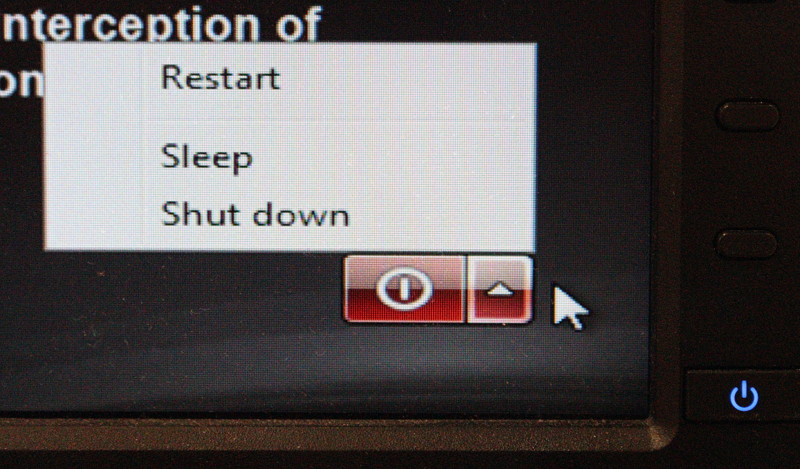
\includegraphics[width=15cm]{images/TH-shutdown-win}}
\caption{Restarting the PC}
\label{figure:welc-restart}
\end{figure}

The system will shut down and we'll be back to the boot selection menu
screen we saw earlier in Figure~\ref{figure:welc-grub}. This time, use
the up/down arrow keys to select \ttout{EPS Linux (Scientific
  Linux)}. Linux will now start, and after a short while you should
see a black screen, with a white login prompt. We won't login to Linux
at this stage, that can wait until a later lab, next week. We would,
however, like you to read the rest of this document, which gives you
some useful and interesting background information about Linux. If you
don't have time to finish reading it in the lab, please make sure you
do so before the next lab session.

\section{Using the School Linux system}

Over the next couple of weeks you will be undertaking a number of
introductory labs to familiarise yourself with the School's computing
infrastructure. Much of this is based on devices and machines running Linux, a
variant of the Unix family of operating systems; this document
provides some background on Unix and explains why we think it is
important. It would very useful if you could read this before you
attend the first introductory labs, where the emphasis will be on
leading you through a series of tasks to explore our setup.

\section{Operating Systems}

An \wikipedia{Operating_system}{operating system} (OS) is a suite of
software that makes computer hardware usable; it makes the `raw
computing power' of the hardware available to the user. You're
probably most familiar with
the \wikipedia{Microsoft_windows}{Microsoft Windows} and
Apple \wikipedia{OS_X}{OS X} families of operating systems for
`desktop' computers, and \wikipedia{Ios}{iOS} (Apple, again) and
Google's \wikipedia{Android_(operating_system)}{Android} for mobile
devices; but many other more specialist operating systems exist, and
you'll be studying some of these and the principles that underpin OS
design in COMP25111 in your second year. In the meantime, a potted
history of OS development will tide us over\ldots
 
\section{Unix Origins}
\label{sec:unix}

In the late 1950s, an American company
called \wikipedia{Bell_Labs}{Bell Laboratories} decided that they
needed a system to improve the way they worked with their computer
hardware (it's probably quite hard to imagine what interacting with a
computer \emph{without} an operating system might be; but it wasn't
pretty and involved manually loading and running programs one by
one). Together with the \wikipedia{General_Electric_Company}{General
Electric Company} and the \wikipedia{MIT}{Massachusetts Institute of
Technology}, they set about the design of an operating system they
called \wikipedia{Multics}{Multics}: the `Multiplexed Information and
Computing Service'. Multics was hugely innovative, and introduced many
concepts that we now take for granted in modern operating systems such
as the ability for more than one program to run `at once'; but it did
rather suffer from `design by committee', and the final system was
seen at the time as being overly complex and rather bloated (`bloated'
is all a matter of perspective of course: its sobering to realise
though that the entire Multics operating system was only around
135Kb. Today's operating systems are something like 30,000 times this
size\ldots). In the late 1960s, a group of programmers at Bell Labs
created a cut-down, leaner and cleaner version of Multics that would
work on more modest hardware. Legend has it that this was to allow
them to play their favourite (only!) computer
game, \wikipedia{Space_Travel_(video_game)}{Space Travel}. In an early
example of the trend of giving things `punny' names, to contrast with
the more clumsy Multics, they called this new system Unix. The
so-called \wikipedia{Jargon_File}{Jargon File} is a good source of
explanations of various bits of computer slang and their obscure
origins, and is well worth a read: in part to give some background
history, but mostly as an insight into the minds of the computing
pioneers of the past!

%\begin{htmlonly}
%(See the Unix entry in the useful and amusing
%\htmladdnormallink{Jargon
%file}{http://www.new.ox.ac.uk/admin/jargon/html/entry/Unix.html}, a
%file}{http://www.cs.manchester.ac.uk/software/jargon/html/entry/Unix.html}, a
%file}{\jargonFileUnix}, a
%`collection of slang terms used by various subcultures of computer
%\htmladdnormallink{hackers}
%{http://www.cs.manchester.ac.uk/software/jargon/html/entry/hacker.html}'.)
%{\jargonFileHackers}'.)
%\end{htmlonly}

Even though Unix is now quite old, most Computer Scientists recognise that the designers of Unix got most of the fundamental concepts and
architecture right. Given how much computing has changed since the 1960s, this was an astonishing intellectual achievement. Although Microsoft's \wikipedia{Microsoft_Windows}{Windows} is by far the most common operating system on \emph{desktop} machines, the majority of the Internet, much of the world's corporate infrastructure, virtually all supercomputers, and even some mobile devices are powered by Unix-like operating systems. So, while the polished graphical user interfaces of Windows and \wikipedia{OS_X}{OS X} appear to dominate the world of computing, most of the real hard-core and leading-edge computation relies on an elegant operating system designed nearly 50 years ago (by a team of scientists who wanted to play a game).  

\section{Modern Unix Variants}
\label{sec:modern-unix-variants}


The history of Unix is complex and convoluted, with the system being updated, re-implemented, and mimicked repeatedly over the years, primarily by commercial companies who guarded their versions jealously. Figure \ref{fig:unix-history} shows a tiny fragment of the Unix's `family tree' (the full diagram, which you can find at \urlnop{www.levenez.com/unix/unix.pdf}, is \emph{many} times the size of the portion you can see here).

\begin{figure}[h!tb]
  \begin{center}
    \includegraphics[width=13cm]{images/unix}
  \end{center}
\caption{A fragment of \'{E}ric L\'{e}v\'{e}nez's Unix History chart, reproduced with permission and showing the beginnings of Linux in amongst other versions of Unix.}
\label{fig:unix-history}
\end{figure}
 
Although many of the branches represent interesting innovations of one kind or another, there are perhaps two that deserve particular attention. The first of these was the decision by Apple some time around the turn of the millennium to drop their own---highly popular, but ageing---bespoke operating system (unimaginatively called \wikipedia{Mac_os_9}{Mac OS 9}) in favour of a Unix-based system (now the more familiar `OS X', where `X' is both the Roman numeral `10' and a nod in the direction of the uniX nature of the OS). Although the majority of Mac users are blissfully unaware of the fact, behind the slick front-end of OS X, sits a variant of Unix. The second, and perhaps more profound of these events was the creation in 1991 by Swedish programmer \wikipedia{Linus_torvalds}{Linus Torvalds} of a Unix-like system, the source code to which \emph{he gave away for free}\footnote{`free' here in the sense both of `freedom to reuse or adapt', and also in the sense of `without charge'.}; this became known as the \wikipedia{Linux_kernel}{Linux Kernel}. Combined with other free software created by the \wikipedia{Free_software_foundation}{Free Software Foundation}, a non-commercial version of Unix called \wikipedia{GNU/Linux}{GNU/Linux} was born (GNU here is a recursive acronym for ``GNU's not Unix'', a swipe at other commercial non-Free versions; much to the annoyance of the Free Software Foundation, GNU/Linux is almost always called just `Linux'\footnote{Linux
is pronounced ``Linn-ucks'', despite the fact the name was coined by
its creator, and his name `Linus' is pronounced
``Leen-uss''!}.) 

Linux has been, and continues to be, developed cooperatively by
thousands of programmers across the world contributing their effort
largely free of charge. It is amazing to think that such
a project could ever happen---and it is surely a testament to the
better side of Human nature. But what is interesting is the
observation that these programmers are not motivated by commercial
concerns, but by the desire to make good reliable software and have it
used by lots of people. Thus, Linux is a good choice of Unix: it's
Free, it's efficient, and it's reliable, and it is now used by large corporations, governments, research labs and individuals around the world. Even Google's \wikipedia{Android_(operating_system)}{Android} platform is a Linux-based mobile OS, and the  \wikipedia{Amazon_Kindle}{Amazon Kindle} is also a Linux box behind the electronic ink of its user interface (Figure \ref{fig:kindlelinux}).

\begin{figure}[h!tb]
  \begin{center}
    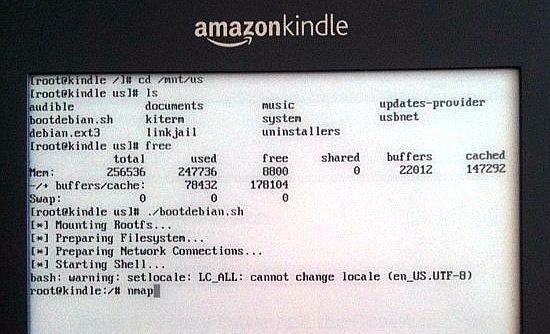
\includegraphics[width=13cm]{images/kindleroot}
  \end{center}
\caption{A photograph of Liraz Siri's `rooted' kindle, showing the Linux command prompt. Reproduced with the author's kind permission from \urlnop{www.turnkeylinux.org/blog/kindle-root}}
\label{fig:kindlelinux}
\end{figure}

One of the results of the fact that Linux is Free is that several
organisations and companies have created their own distributions of
it; these vary a bit (in fact, anybody is free to make any change they
like to Linux, and pass it on to whoever wants it). The distribution
we use in this School is \textbf{Fedora}, which is
one of the most popular and is sponsored by a
US company called \textbf{Red Hat}.
%, which is the latest release

So, if you are to become an expert computer professional, it is
important that you understand the theory and practice of Unix based
systems. Learning Unix is not only a crucial skill for any serious
computer scientist, it is a very rewarding experience; the labs over
the next couple of weeks are designed to help you become familiar with what will be your daily working environment.

